\section{572 --- Subtree of Another Tree}
Given two non-empty binary trees $s$ and $t$, check whether tree $ t $ has exactly the same structure and node values with a subtree of $ s $. A subtree of $ s $ is a tree consists of a node in $ s $ and all of this node's descendants. The tree $ s $ could also be considered as a subtree of itself.

\paragraph{Example 1:}
\begin{flushleft}
\textbf{Input}:
Given tree $s$:
\begin{figure}[H]
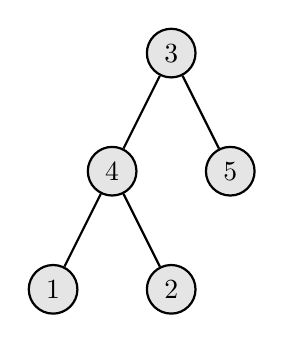
\begin{tikzpicture}
[every node/.style={draw, circle,minimum size=6mm, fill=gray!20!},
  node distance=8mm, thick]
\node{3}
child{node{4} child{node{1}} child{node{2}}}
child{node{5}};
\end{tikzpicture}
\end{figure}

Given tree $t$:

\begin{figure}[H]
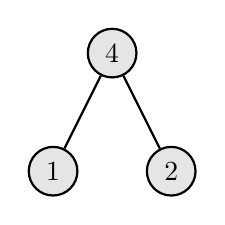
\begin{tikzpicture}
[every node/.style={draw, circle,minimum size=6mm, fill=gray!20!},
  node distance=8mm, thick]
\node{4} 
child{node{1}}
child{node{2}};
\end{tikzpicture}
\end{figure}

\textbf{Output}: \texttt{true}

\textbf{Explanation}: because $t$ has the same structure and node values with a subtree of $s$.
\end{flushleft}

\paragraph{Example 2:}

\begin{flushleft}
Given tree $s$:
\begin{figure}[H]
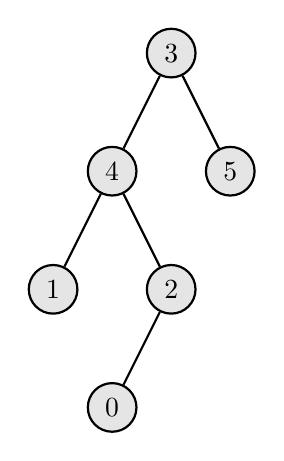
\begin{tikzpicture}
[every node/.style={draw, circle,minimum size=6mm, fill=gray!20!},
  node distance=8mm, thick]
\node{3}
child{node{4} child{node{1}} child{node{2} child{node{0}} child[missing]}}
child{node{5}};
\end{tikzpicture}
\end{figure}

Given tree $t$:
\begin{figure}[H]
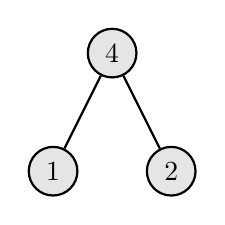
\begin{tikzpicture}
[every node/.style={draw, circle,minimum size=6mm, fill=gray!20!},
  node distance=8mm, thick]
\node{4} 
child{node{1}}
child{node{2}};
\end{tikzpicture}
\end{figure}

\textbf{Output}: \texttt{false}
\end{flushleft}

\subsection{Recursion}
\begin{itemize}
\item We need a helper function to check if two binary tree are equal, i.e., they have same structure and values.
\item In the main function, first we check if the binary tree rooted with $s$ is equal to $t$ or not. If they are equal, just return \texttt{true}. Otherwise, we recursively call the main function to compare left/right child tree of $s$ against $t$. If either case return \texttt{true}, we just return \texttt{true}.
\item We do not call the helper function to recursively compare left/right child tree of $s$ against $t$. The reason is that helper function only check two trees with fixed root. For example, if left child tree of $s$ is not equal to $t$, the helper function will not recursively to try the left grandchild or right grandchild of $s$.
\end{itemize}

\setcounter{lstlisting}{0}
\begin{lstlisting}[style=customc, caption={Recursion}]
bool isSubtree( TreeNode* s, TreeNode* t )
{
    if( equal( s, t ) )
    {
        return true;
    }

    if( s )
    {
        //compare left/right child of s to t
        return isSubtree( s->left, t ) || isSubtree( s->right, t );
    }

    return false;
}

//helper function to check if s and t
//has same structure and node values.
//s and t are fixed.
bool equal( TreeNode* s, TreeNode* t )
{
    if( !s && !t )
    {
        return true;
    }

    if( !s || !t )
    {
        return false;
    }

    if( s->val == t->val )
    {
        return equal( s->left, t->left ) && equal( s->right, t->right );
    }

    return false;
}
\end{lstlisting}